\documentclass[12pt]{amsart}
\usepackage{amsmath,enumerate,commath,tikz}
\usetikzlibrary{angles,quotes}
\openup 5pt
\author[Blake Farman]{Blake Farman\\University of South Carolina}
\title[Exam 01]{Math 142: Exam 01}
\date{February 13, 2018}
\pdfpagewidth 8.5in
\pdfpageheight 11in
\usepackage[margin=1in]{geometry}

\renewcommand{\qedsymbol}{}

\begin{document}
\maketitle

\begin{center}
  \fbox{\fbox{\parbox{5.5in}{\centering
        Answer the questions in the spaces provided on the
        question sheets and turn them in at the end of the class period.

        Unless otherwise stated, all supporting work is required.
        Unsupported or otherwise mysterious answers will \textbf{not receive credit.}
        
        You may \textbf{not} use a calculator or any other electronic device, including cell phones, smart watches, etc.
        By writing your name on the line below, you indicate that you have read and understand these directions.


        It is advised, although not required, that you check your answers.}}}
\end{center}

\vspace{0.2in}
\makebox[\textwidth]{Name:\enspace\hrulefill}
\vspace{0.2in}

\theoremstyle{definition}
\newtheorem{thm}{}
\renewcommand{\qedsymbol}{}

\[
\begin{array}{|c|c|c|}
  \hline
  \text{Problem} & \text{Points Earned} & \text{Points Possible}\\
  \hline
  1 & & 20\\
  \hline
  2 & & 20\\
  \hline
  3 & & 20\\
  \hline
  4 & & 20\\
  \hline
  5 & & 20 \\
  \hline
%  \text{Bonus} & & 10\\
%  \hline
  \text{Total} & & 100\\
  \hline
\end{array}
\]

\newpage

\section{Problems}

For each of the following problems, decide which method of integration is appropriate and compute the given integrals.

\begin{thm}[20 Points]
  Compute 
    \(\displaystyle{\int \cos^2(\theta)\sin^2(\theta)\dif \theta}\).
    %\vspace{3in}
\end{thm}
\begin{proof}[Solution]
  We use the identities
  \[\sin^2(\theta) = \frac{1 - \cos(2\theta)}{2}\ \text{and}\ \cos^2(\theta) = \frac{1 + \cos(\theta)}{2}\]
  to rewrite the integrand as
  \begin{eqnarray*}
    \sin^2(\theta)\cos^2(\theta) &=& \left(\frac{1 - \cos(2\theta)}{2}\right)\left(\frac{1 + \cos(2\theta)}{2}\right)\\
    &=& \frac{1 - \cos^2(2\theta)}{4}\\
    &=& \frac{1}{4}\left(1 - \left(\frac{1 + \cos(4\theta)}{2}\right)\right)\\
    &=& \frac{1}{4} - \frac{1}{8} - \frac{\cos(4\theta)}{8}\\
    &=& \frac{1}{8} -\frac{\cos(4\theta)}{8}\\
    &=& \frac{1}{8}\left(1 - \cos(4\theta)\right)
  \end{eqnarray*}
  Therefore
  \[\int \sin^2(\theta)\cos^2(\theta)\dif \theta = \frac{1}{8}\left(\int \dif\theta -\int \cos(4\theta)\dif\theta\right) = \frac{1}{8}\left(\theta - \frac{\sin(4\theta)}{4}\right) + C\]
\end{proof}

\begin{thm}
  Compute
  \(\displaystyle{\int e^x\cos(x)\dif x}\).
\end{thm}
\begin{proof}[Solution]
      We use integration by parts twice.
      For the first application, we take
      \[\begin{array}{ll}
      u = e^x & v = \sin(x)\\
      \dif u = e^x \dif x & \dif v = \cos(x)\dif x
      \end{array}\]
      to get
      \[\int e^x \cos(x)\dif x = e^x\sin(x) - \int e^x\sin(x)\dif x.\]
      Now we apply integration by parts to \(\int e^x\sin(x)\dif x\) using
      \[\begin{array}{ll}
      u = e^x & v = -\cos(x)\\
      \dif u = e^x \dif x & \dif v = \sin(x)\dif x
      \end{array}\]
      to get
      \[\int e^x\sin(x)\dif x = -e^x\cos(x) - \int e^x(-\cos(x))\dif x = -e^x\cos(x) + \int e^x\cos(x)\dif x.\]
      We note that the this last integral is exactly the integral we started with.
      So, we substitute this into the original equation to find
      \begin{eqnarray*}
        \int e^x\cos(x)\dif x &=& e^x\sin(x) - \left(-e^x \cos(x) + \int e^x\cos(x)\dif x\right)\\
        &=& e^x\sin(x) + e^x\cos(x) - \int e^x\cos(x)\dif x
      \end{eqnarray*}
      then add \(\int e^x \cos(x)\dif x\) to both sides to obtain
      \[2 \int e^x\cos(x)\dif x = e^x \sin(x) + e^x \cos(x).\]
      Dividing both sides of this equation by two and adding a constant of integration, we have
      \[\int e^x\cos(x) = \frac{e^x\sin(x) + e^x\cos(x)}{2} + C.\]
\end{proof}

%\newpage

\begin{thm}[20 Points]
  Compute \(\displaystyle{\int\frac{\dif x}{\sqrt{x^2 - 9}}}\).
\end{thm}

\begin{proof}[Solution]
  We recall that
  \[\sec^2(\theta) - 1 = \frac{1}{\cos^2(\theta)} - \frac{\cos^2(\theta)}{\cos^2(\theta)} = \frac{1 - \cos^2(\theta)}{\cos^2(\theta)} = \frac{\sin^2(\theta)}{\cos^2(\theta)} = \tan^2(\theta).\]
  Since the integrand is only real valued for \(3 < x\), we can make the trigonometric substitution \(x = 3\sec(\theta)\) for \(0 < \theta < \pi/2\).
  As tangent is positive for these values of \(\theta\), the denominator becomes
  \[\sqrt{x^2 - 9} = \sqrt{9\sec^2(\theta) - 9} = \sqrt{9(\sec^2(\theta) - 1)} = \sqrt{9\tan^2(\theta)} = 3\tan(\theta).\]
  We compute
  \[\dif x = 3\tan(\theta)\sec(\theta) \dif\theta\]
  and so
  \[\int \frac{\dif x}{\sqrt{x^2 - 9}} = \int \frac{3\tan(\theta)\sec(\theta)\dif\theta}{3\tan(\theta)} = \int \sec(\theta)\dif\theta = \ln(\sec(\theta) + \tan(\theta)) + C\]
  since \(0 < \theta < \pi/2\) implies that both \(\sec(\theta)\) and \(\tan(\theta)\) are positive.

  To get to our answer in terms of \(x\) we note that
  \[\frac{x}{3} = \sec(\theta) = \frac{1}{\cos(\theta)}\]
  so we look at the right triangle
  \begin{center}
    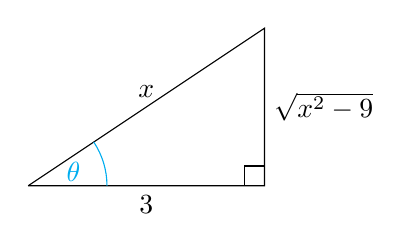
\begin{tikzpicture}[
        my angle/.style={
          every pic quotes/.append style={text=cyan},
          draw=cyan,
          angle radius=1cm,
      }]
      \coordinate (C) at (-1.5,-1);
      \coordinate (A) at (1.5,-1);
      \coordinate (B) at (1.5,1);
      \draw (C) -- node[above] {$x$} (B) -- node[right] {$\sqrt{x^2 - 9}$} (A) -- node[below] {$3$} (C);
      \draw (A) +(-.25,0) |- +(0,.25);
      \pic [my angle, "$\theta$"] {angle=A--C--B};
      %\pic [my angle, "$\beta$"] {angle=C--B--A};
    \end{tikzpicture}
  \end{center}
  to see that \(\tan(\theta) = \frac{\sqrt{x^2 - 9}}{3}\).
  Therefore
  \[\int \frac{\dif x}{\sqrt{x^2 - 9}} = \ln\left(\frac{x}{3} + \frac{\sqrt{x^2 - 9}}{3}\right) + C\]
\end{proof}

%\newpage

\begin{thm}[20 Points]
  Compute \[\int \frac{6x^2 - 2}{(x + 1)(x - 1)(x^2 + 1)}\dif x\].
\end{thm}

\begin{proof}[Solution]
  First we set up the equation
  \[\frac{6x^2 - 2}{(x + 1)(x - 1)(x^2 + 1)} = \frac{A}{x+1} + \frac{B}{x - 1} + \frac{Cx + D}{x^2 + 1}\]
  then multiply both sides \(x+1)(x - 1)(x^2 + 1)\) to get
  \begin{eqnarray*}
    6x^2 - 2 &=& A(x - 1)(x^2 + 1) + B(x + 1)(x^2 + 1) + (Cx + D)(x^2 - 1)\\
    &=& A(x^3 - x^2 + x - 1) + B(x^3 + x^2 + x + 1) + Cx^3 + Dx^2 - Cx - D\\
    &=& (A + B + C)x^3 + (-A + B + D)x^2 + (A + B - C)x + (-A + B -D).
  \end{eqnarray*}
  Equating the coefficients gives the system
  \begin{eqnarray*}
    0 &=& A + B + C\\
    6 &=& -A + B + D\\
    0 &=& A + B - C\\
    -2 &=& -A + B - D\\
  \end{eqnarray*}
  Adding the first and third equations together gives \(2A + 2B = 0\), which is equivalent to \(A + B = 0\).
  This implies that \(B = -A\) and hence \(C = 0\).
  Subtracting the fourth equation from the second equation gives
  \[8 = (-A + B + D) - (-A + B - D) = -(A + B) + (A + B) + D + D = 2D\]
  so we see that \(D = 4\).
  Plugging \(D = 4\) and \(B = -A\) into the second equation gives
  \(6 = B + B + 4 = 2B + 4\)
  and thus
  \[B = \frac{6 - 4}{2} = \frac{2}{2} = 1.\]
  Therefore the solution to the system is \(A = -1, B = 1, C = 0, D = 4\) and
  \begin{eqnarray*}
    \int \frac{6x^2 - 2}{(x + 1)(x - 1)(x^2 + 1)}\dif x &=& -\int\frac{\dif x}{x + 1} + \int \frac{\dif x}{x - 1} + 4\int\frac{dx}{x^2 + 1}\\
    &=& -\ln\abs{x + 1} + \ln\abs{x - 1} + 4\arctan{x} + C
  \end{eqnarray*}
\end{proof}
%\newpage

\begin{thm}[20 Points]
  Decide whether 
  \[\int_2^\infty \frac{\dif x}{x^2 - 1}\]
  converges or diverges.
  If it converges, find the value of the integral.
\end{thm}

\begin{proof}[Solution]
  By definition we have
  \[\int_2^\infty \frac{\dif x}{x^2 - 1} = \lim_{t \to \infty} \int_2^t \frac{\dif x}{x^2 - 1}.\]
  Factoring the denominator as \(x^2 - 1 = (x + 1)(x - 1)\) we can do the definite integral by partial fraction decomposition as follows.
  Set
  \[\frac{1}{(x - 1)(x + 1)} = \frac{A}{x - 1} + \frac{B}{x + 1}\]
  then clear denominators to get
  \[1 = A(x + 1) + B(x - 1) = (A + B)x + (A - B)\]
  and equate coefficients to obtain the system
  \begin{eqnarray*}
    0 &=& A + B\\
    1 &=& A - B.
  \end{eqnarray*}
  Adding the two equations together gives \(1 = 2A\), while subtracting the second equation from the first gives \(-1 = 2B\).
  Thus \(A = 1/2\), \(B = -1/2\), and
  \begin{eqnarray*}
    \lim_{t \to \infty} \int_2^t \frac{\dif x}{x^2 - 1} &=& \lim_{t \to \infty}\left(\frac{1}{2}\int_2^t \frac{\dif x}{x - 1} - \frac{1}{2} \int_2^t \frac{\dif x}{x + 1}\right)\\
    &=& \lim_{t \to \infty} \left(\frac{1}{2}\left[\ln \abs{x - 1} - \ln\abs{x+1}\right]_2^t\right)\\
    &=& \lim_{t \to \infty} \left(\frac{\ln \abs{t - 1} - \ln\abs{t + 1} - \ln(2 - 1) + \ln(2 + 1)}{2}\right)\\
    &=& \lim_{t \to \infty} \frac{1}{2}\left(\ln\abs{\frac{t - 1}{t + 1}} + \ln(3)\right).
  \end{eqnarray*}
  Since both the natural logarithm and the absolute value functions are continuous we have 
  \[\lim_{t \to \infty} \ln\abs{\frac{t - 1}{t + 1}} = \ln\left(\lim_{t \to \infty} \abs{\frac{t -  1}{t + 1}}\right) = \ln\abs{\lim_{t\to\infty} \frac{t -1}{t + 1}} = \ln(1) = 0.\]
  Therefore
  \[\int_2^\infty \frac{\dif x}{x^2 - 1} =  \lim_{t \to \infty} \frac{1}{2}\left(\ln\abs{\frac{t - 1}{t + 1}} + \ln(3)\right) = \frac{0 + \ln(3)}{2} = \frac{\ln(3)}{2}.\]
\end{proof}

\begin{proof}[Alternate Solution]
  This solution is much more difficult, in my opinion, but I include it becuase quite a few folks attempted this problem in this way.

  We first make a couple of observations.
  The first is that
  \[\frac{\dif}{\dif \theta} \csc(\theta) = \frac{\dif}{\dif \theta} \sin(\theta)^{-1} = -\sin(\theta)^{-2} \frac{\dif}{\dif \theta} \sin(\theta) = -\frac{\cos(\theta)}{\sin^2(\theta)} = -\cot(\theta)\csc(\theta).\]
  The second observation is that
  \[\frac{\dif}{\dif \theta} \cot(\theta) = \frac{\dif}{\dif \theta} \tan(\theta)^{-1} = -\tan(\theta)^{-2} \frac{\dif}{\dif \theta} \tan(\theta) = \frac{\sec^2(\theta)}{\tan^2(\theta)} = \frac{1}{\cos^2(\theta)}\frac{\cos^2(\theta)}{\sin^2(\theta)} = -\csc^2(\theta).\]
  Combining these two together we have the important observation, which will come in handy later:
  \[\frac{\dif}{\dif \theta}(\csc(\theta) + \cot(\theta)) = -\cot(\theta)\csc(\theta) - \csc^2(\theta) =-\csc(\theta)(\cot(\theta) + \csc(\theta))\]

  With these observations in hand, we can forge ahead with a trigonometric substition \(x = \sec(\theta)\), so that \(x^2 - 1 = \sec^2(\theta) - 1 = \tan^2(\theta)\), and \(\dif x = \sec(\theta)\tan(\theta)\dif{\theta}\).
  The indefinite integral we will need to compute is
  \begin{eqnarray*}
    \int \frac{\dif x}{x^2 - 1} &=& \int \frac{\sec(\theta)\tan(\theta)}{\tan^2(\theta)}\dif{\theta}\\
    &=& \int \frac{\sec(\theta)}{\tan(\theta)}\dif{\theta}\\
    &=& \int \frac{1}{\cos(\theta)}\frac{\cos(\theta)}{\sin(\theta)}\dif{\theta}\\
    &=& \int \frac{1}{\sin(\theta)}\dif{theta}\\
    &=& \int \csc(\theta)\dif{\theta}\\
  \end{eqnarray*}
  This is where we use our main observation above: take \(u = \csc(\theta) + \cot(\theta)\) so that \(-\dif{u} = \csc(\theta)(\csc(\theta) + \cot(\theta))\) and then
  \begin{eqnarray*}
    \int \csc(\theta) \dif{\theta} &=& \int \frac{\csc(\theta)(\csc(\theta) + \tan(\theta))}{\csc(\theta) + \cot(\theta)}\dif{\theta}\\
    &=& -\int \frac{\dif{u}}{u}\\
    &=& -\ln\abs{\csc(\theta) + \cot(\theta)} + C
  \end{eqnarray*}
  Now, we can look at the triangle
  \begin{center}
    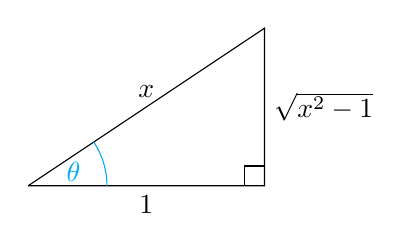
\begin{tikzpicture}[
        my angle/.style={
          every pic quotes/.append style={text=cyan},
          draw=cyan,
          angle radius=1cm,
      }]
      \coordinate (C) at (-1.5,-1);
      \coordinate (A) at (1.5,-1);
      \coordinate (B) at (1.5,1);
      \draw (C) -- node[above] {$x$} (B) -- node[right] {$\sqrt{x^2 - 1}$} (A) -- node[below] {$1$} (C);
      \draw (A) +(-.25,0) |- +(0,.25);
      \pic [my angle, "$\theta$"] {angle=A--C--B};
      %\pic [my angle, "$\beta$"] {angle=C--B--A};
    \end{tikzpicture}
  \end{center}
  to rewrite our solution in terms of \(x\) as
  \begin{eqnarray*}
    \int \frac{\dif{x}}{x^2 - 1} &=& -\ln\left(\frac{x}{\sqrt{x^2 - 1}} + \frac{1}{\sqrt{x^2 - 1}}\right) + C\\
    &=& -\ln\left(\frac{x + 1}{\sqrt{x^2 - 1}}\right) + C\\
    &=& -\ln\left( \frac{\sqrt{x + 1}\sqrt{x + 1}}{\sqrt{x - 1}\sqrt{x + 1}}\right) + C\\
    &=& -\ln\left(\sqrt{\frac{x + 1}{x - 1}}\right) + C\\
    &=& -\frac{1}{2} \ln\left(\frac{x + 1}{x -1}\right) + C
  \end{eqnarray*}
  keeping in mind that we are only interested in \(2 \leq x\). 

  Now we can evaluate the improper integral
  \begin{eqnarray*}
    \int_2^\infty \frac{\dif x}{x^2 - 1} &=& \lim_{t \to \infty} \int_2^t \frac{\dif x}{x^2 - 1} = \lim_{t \to \infty} -\frac{1}{2}\left[\ln\left(\frac{x + 1}{x - 1}\right)\right]_2^t\\
    &=& \lim_{t \to \infty} -\frac{1}{2}\left(\ln\left(\frac{t + 1}{t - 1}\right) - \ln\left(\frac{2 + 1}{2 - 1}\right)\right)\\
    &=& \lim_{t \to \infty} \frac{1}{2}\left(\ln(3) - \ln\left(\frac{t + 1}{ t - 1}\right)\right)\\
    &=& \frac{1}{2}(\ln(3) - 0)\\
    &=& \frac{\ln(3)}{2}.
  \end{eqnarray*}
\end{proof}

%\newpage

%\begin{thm}[Joke - 5 Points]
%  Infinitely many mathematicians walk into a bar.
%  The \(\text{zero}^\text{th}\) mathematician orders a beer, the first mathematician tells the barkeep \lq I'll have half of what he had,\rq\ the second mathematician tells the barkeep \lq I'll have half of what he had,\rq\ and so on.
%  \begin{enumerate}[(a)]
%  \item
%    Write down an exponential function, \(f\), that models the setup.
%    That is, \(f(0) = 1\), \(f(1) = 1/2\), etc.
%  \item
%    The barkeep becomes fed up with the mathematicians.
%    Having taken Math 142 previously, he pours two pints, sets them on the bar and tells the mathematicians, \lq You sort it out amongst yourselves.\rq

%    Decide whether the barkeep has poured enough beer for all the mathematicians.
%    Justify your answer.\\
%    {[Hint: \(1/\ln(2) \approx 1.44\).]}
%  \end{enumerate}
%\end{thm}

\end{document}
